{

\subsubsection{Metode}
Floodfill finder i sin enkelthed områder i et billede, som har en farve
der ligger inde for en vis afvigelse af den originale farve. Der vælges
en pixel i billedet som har en farve angivet ved en RGB-værdi. Ud fra
denne pixel findes de fire tilstødende pixels i lodret og vandret bane,
som vist i figur \ref{floodfill1}.

\begin{figure}[!h]
    \begin{center}
        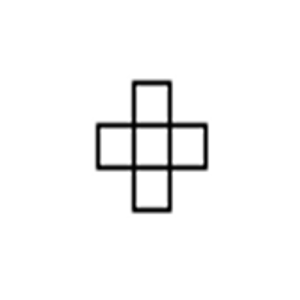
\includegraphics[scale=0.42,angle=0]{afsnit/vores_implementation/billeder/flood_fill/floodfill1}
    \end{center}
    \caption[]{Måden floodfill arbejder med pixels i billedet}
    \label{floodfill1}
\end{figure}

De følgende 3 skridt beskriver hvordan floodfillmetoden virker i et
billede.
\begin{enumerate}
    \item Algoritmen starter med at markere den midterste pixel (vores
        startpixel) med et rødt flag, som angiver at denne pixel bliver
        farvet. Nabopixels får et blåt flag, som angiver at de skal
        kontrolleres for om deres farve er indenfor afvigelsen. Blå flag
        sættes kun hvis en pixel ikke har noget flag i forvejen. Se
        figur \ref{floodfill2}.
    \item Hver pixel med et blåt flag kontrolleres for om deres
        farve ligger indenfor afvigelsen. Hvis farven er indenfor
        afvigelsen, bliver denne pixel sat i en liste og markeret med et
        grønt flag og et tal. Se figur \ref{floodfill3}
    \item En pixel med grønt flag tages ud af listen og bliver sat til
        den nye startpixel. Skridt $1$ og $2$ bliver gentaget til der
        ikke er flere grønne flag. Se figur \ref{floodfill4}
\end{enumerate}

\begin{figure}[!h]
    \begin{center}
        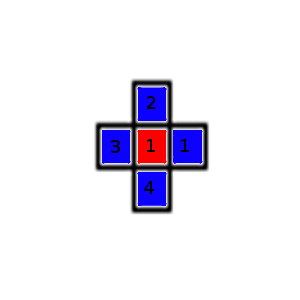
\includegraphics[scale=0.42,angle=0]{afsnit/vores_implementation/billeder/flood_fill/floodfill2}
    \end{center}
    \caption[]{Pixels efter første skridt i algoritmen. Den røde pixels
    er vores startpixel. Pixels markeret med blåt skal kontrolleres for
    deres farve. Numrene angiver rækkefølgen de bliver gennemgået.}
    \label{floodfill2}
\end{figure}

\begin{figure}[!h]
    \begin{center}
        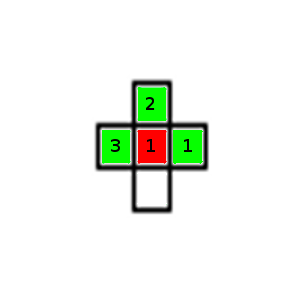
\includegraphics[scale=0.42,angle=0]{afsnit/vores_implementation/billeder/flood_fill/floodfill3}
    \end{center}
    \caption[]{Pixels efter andet skridt i algoritmen. De pixels som har
    en farve der ligger indenfor afvigelsen bliver markeret med et grønt
    flag og tildelt et tal som angiver rækkefølgen. I denne illustration
    er den nederste pixel ikke blevet farvet grøn. Den var før blå, men
    da den ikke ligger indenfor afvigelsen mister den sit flag, og kan
    komme i betraktning igen, næste gang motoden arbejder ud fra en af
    de pixels som befinder sig op af den}
    \label{floodfill3}
\end{figure}

\begin{figure}[!h]
    \begin{center}
        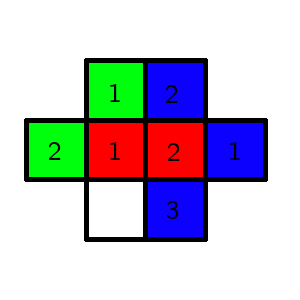
\includegraphics[scale=0.42,angle=0]{afsnit/vores_implementation/billeder/flood_fill/floodfill4}
    \end{center}
    \caption[]{Pixels efter skridt 3 og et nyt skridt 1. Vi har valgt
    den grønne pixel med det laveste tal fra figur \ref{floodfill3} som
    ny startpixel. Nye pixels markeret med blåt mangler at blive
    kontrolleret.}
    \label{floodfill4}
\end{figure}

På denne måde itererer metoden sig igennem alle de pixels som ligger
inde for en vis afgivelse fra startfarven. Denne metode kan gøres på to
måder; Enten kan man regne afvigelsen ud fra farven som vores startpixel
har eller man kan regne den fra den nye pixel som bliver fundet i tredje
skridt.

\subsubsection{Hvilken metode passer best}
Som nævnt ovenfor er der to måder vi kan bruge floodfill på. Hvis man
vælger at regne varianten ud fra den første startpixel vil metoden
indskrænke sig meget og ikke komme ind i alle hjørner af en region. Til
gengæld har denne fremgangsmåde sværere ved at krydse kanter og på den
måde komme ind i en ny region.

Vælger man at ændre varianten efter den nye startpixel vil man male
større regioner. Da denne fremgangsmåde hele tiden tilpasser varianten,
kan man medtage regioner der langsomt skifter farve. Dette er
interessant især med hensyn til digitale billeder af malerier, da solen
eller blitzens refleksion kan påvirke billedet farver. Af samme grund er
den fremgangsmåde heller ikke særlig følsom overfor kanter, hvilket
resulterer i at man let kommer til at gå ind i andre regioner.
Vi har valt at bruge metode nr 2, da i vores mening, giver den
et bedre resultat, da vi menner, at tage højte for sol og smp farve
skift, vægter højer en at være sikker på at den ikke fejler ved at gå ud
over kanterne.

For at få denne metode til at virke på 25000 billeder, hvor en del af
billederne ikke har samme farvetone eller er blevet falmet, må der
for hvert billede udregnes hvad for en varians i farve der skal bruges.
XXX: Stadig intet svar på hvad vi gør!

}

% vim: set tw=72 spell spelllang=da:
